\documentclass[12pt]{article}
\usepackage{hyperref}
\usepackage{graphicx}
\usepackage[T1]{fontenc}
\usepackage[utf8]{inputenc}
\usepackage{color}
\usepackage[font=small,labelfont=bf]{caption}
\usepackage[italian]{babel}
\usepackage{datetime}
\usepackage{fancyhdr}
\usepackage{lastpage}
\usepackage{float}
\pagestyle{fancy}
\fancyhf{}
\rfoot{\center Pagina \thepage \hspace{1pt} di \pageref{LastPage}}
\renewcommand{\today}{\thisdayofweekname\ \the\day\ \monthname\ \the\year}
\title{Analisi sito}
\date{}
\author{Trevisan Davide}
\hypersetup{
	colorlinks=true,       % false: boxed links; true: colored links
	    linkcolor=blue,          % color of internal links (change box color with linkbordercolor)
	    citecolor=green,        % color of links to bibliography
	    filecolor=blue,      % color of file links
	    urlcolor=red,
	    filecolor=red,
	    citecolor=red,
}
\begin{document}
\pagenumbering{arabic}



\begin{titlepage}

\newcommand{\HRule}{\rule{\linewidth}{0.5mm}} % Defines a new command for the horizontal lines, change thickness here

\center % Center everything on the page
 
%----------------------------------------------------------------------------------------
%	HEADING SECTIONS
%----------------------------------------------------------------------------------------

\textsc{\LARGE Università degli Studi di Padova}\\[1.5cm] % Name of your university/college
\textsc{\Large Laurea in Informatica}\\[0.5cm] % Major heading such as course name
\textsc{\large Corso di Tecnlogie Web 2}\\[0.5cm] % Minor heading such as course title

%----------------------------------------------------------------------------------------
%	TITLE SECTION
%----------------------------------------------------------------------------------------

\HRule \\[0.4cm]
{ \huge  Progetto di fine corso}\\[0.3cm] % Title of your document
\HRule \\[1.5cm]
 
%----------------------------------------------------------------------------------------
%	AUTHOR SECTION
%----------------------------------------------------------------------------------------

\begin{minipage}{0.4\textwidth}
\begin{flushleft} \large
\emph{Studente:}\\
Davide Trevisan % Your name
\end{flushleft}
\end{minipage}
~
\begin{minipage}{0.4\textwidth}
\begin{flushright} \large
\emph{Matricola:} \\
\textsc{1070686} % Supervisor's Name
\end{flushright}
\end{minipage}\\[1cm]

% If you don't want a supervisor, uncomment the two lines below and remove the section above
%\Large \emph{Author:}\\
%John \textsc{Smith}\\[3cm] % Your name

%----------------------------------------------------------------------------------------
%	DATE SECTION
%----------------------------------------------------------------------------------------

{\large \today}\\[1cm] % Date, change the \today to a set date if you want to be precise

%----------------------------------------------------------------------------------------
%	LOGO SECTION
%----------------------------------------------------------------------------------------


\includegraphics[scale=0.20]{Logo.png} % Include a department/university logo - this will require the graphicx package
 
%----------------------------------------------------------------------------------------

\vfill % Fill the rest of the page with whitespace

\end{titlepage}

\newpage
\renewcommand{\contentsname}{Indice}
\tableofcontents

\newpage
\pagenumbering{arabic}

\section{Introduzione}
Il documento si propone di fornire una analisi di usabilità (delle pagine principali, data la mole di pagine) del sito \url{http://www.metacritic.com/}, un noto sito americano che si occupa di recensioni di film, serie, album musicali e videogiochi. Si propone di essere un'evoluzione di Rotten Tomatoes, proponendo una copertura di più prodotti. Il sito fornisce per ogni prodotto, se sono presenti più di quattro recensioni, una media del voto pesata, chiamata \textit{metascore}, dividendo le recensioni tra quelle di recensori professionisti e quelle degli utenti che possono registrarsi al sito. Maggiori informazioni su come è ottenuto il \textit{metascore} sono contenute nella pagina \url{http://www.metacritic.com/about-metascores}.\\
Soprattutto nell'ambito dei videogiochi questo sito è considerato come il sito di riferimento per quanto riguarda la valutazione, tanto che la media di metacritic è la valutazione presa per riferimento nell'ambito dei videogiochi e influenza non di poco il volume di vendite di un videogioco.
\\ \\ \textbf{Nota: La presente analisi di usabilità è stata redatta nel periodo di fine giugno 2016, quindi i contenuti del sito potrebbero essere cambiati nel tempo.}
\section{nome del sito}
Il sito non inizia per vocale o per alcuna delle consonanti viste a lezione che comporterebbero un bonus, tuttavia fa uso del favorevole dominio \textit{.com}. La parola \textit{metacritic} inoltre è un neologismo risultante dalla composizione del prefisso greco meta (che significa "oltre") e dalla parola inglese "critc", alludendo al processo di aggregazione di recensioni compiuto dal sito
\newpage
\section{Analisi di usabilità della homepage}
\subsection{A prima vista}
Procediamo innanzitutto ad analizzare la pagina principale. Di seguito viene fornito uno screen della home page così come appare senza l'uso di \textit{adblock}. Per arrivare alla fine servono 3 scroll completi (con uno schermo dalla definizione di 1680x1050). La pagina completa è invece visibile in \href{home1.png}{home1.png}
\begin{figure}[H]
\begin{center}
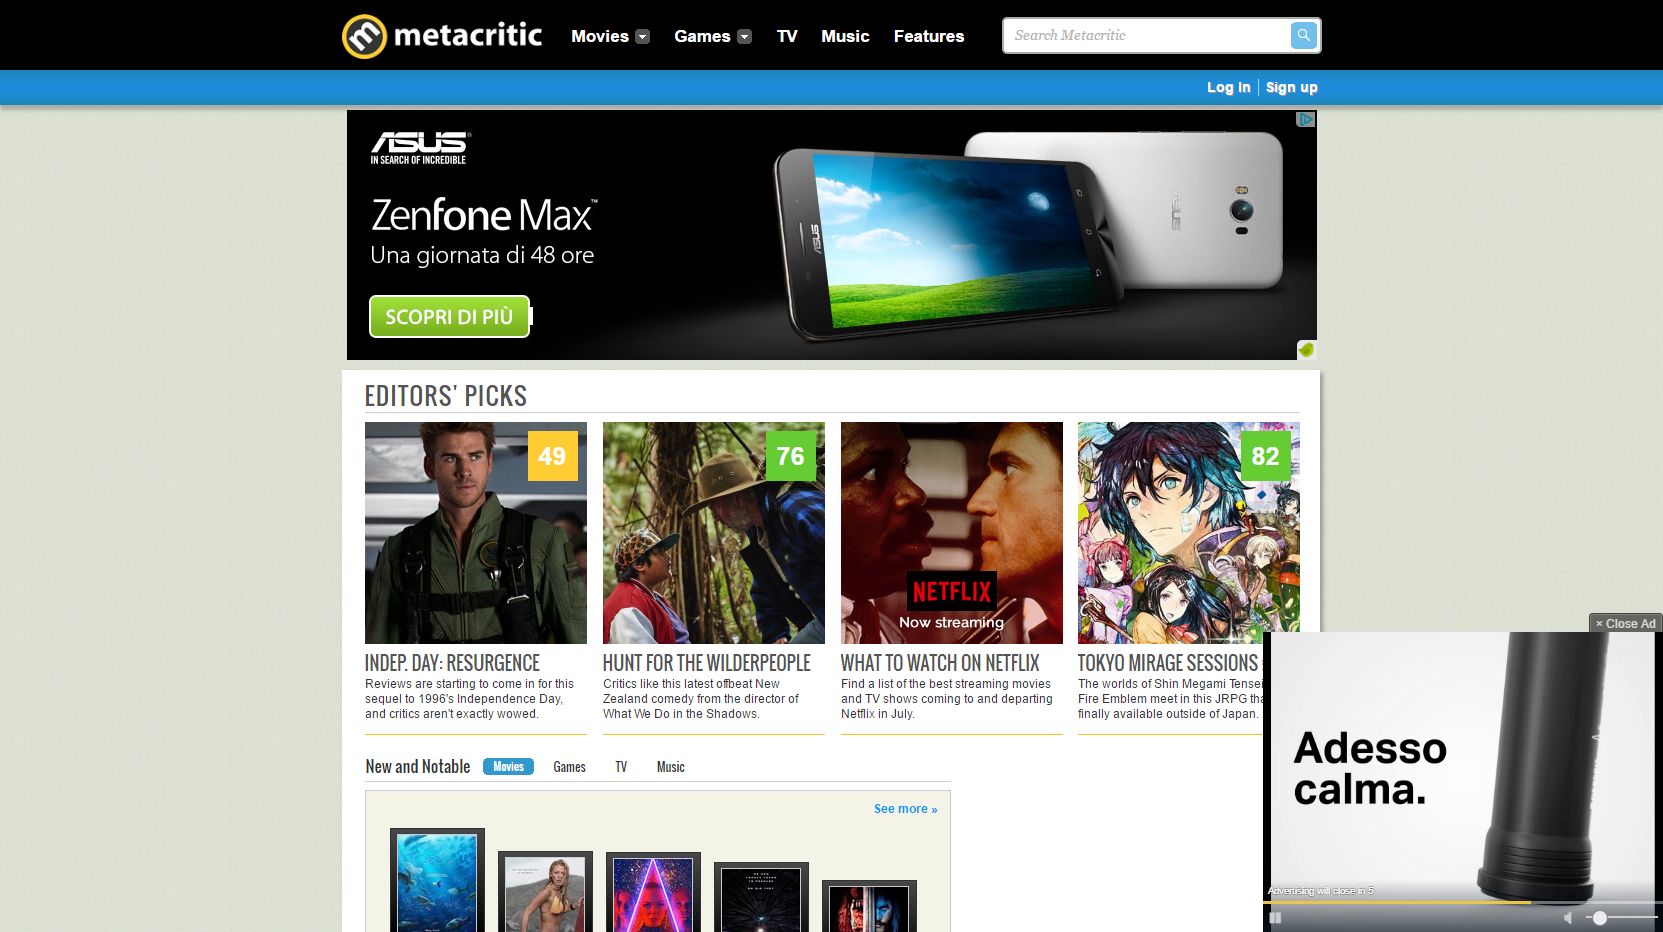
\includegraphics[width=13.5cm]{home.png}
\caption{Home, vedi file \href{home.png}{home.png}}
\end{center}
\end{figure}
Come si può notare il fattore di forma particolare dello schermo contribuisce a lasciare poco spazio alla visualizzazione di contenuto interessante, rendendo obbligatorio lo scrolling. Cosa molto negativa è inoltre il fatto che la lista dei nuovi prodotti con recensione è completamente invisibile.
La presentazione è cmq abbastanza minimale e gradevole alla vista, in quanto non si è caduti in un design eccessivamente pesante.
La situazione migliora nelle homepage delle varie categorie, ad esempio games. La pagina intera è visibile in \href{home21.png}{home21.png}:
\begin{figure}[H]
	\begin{center}
		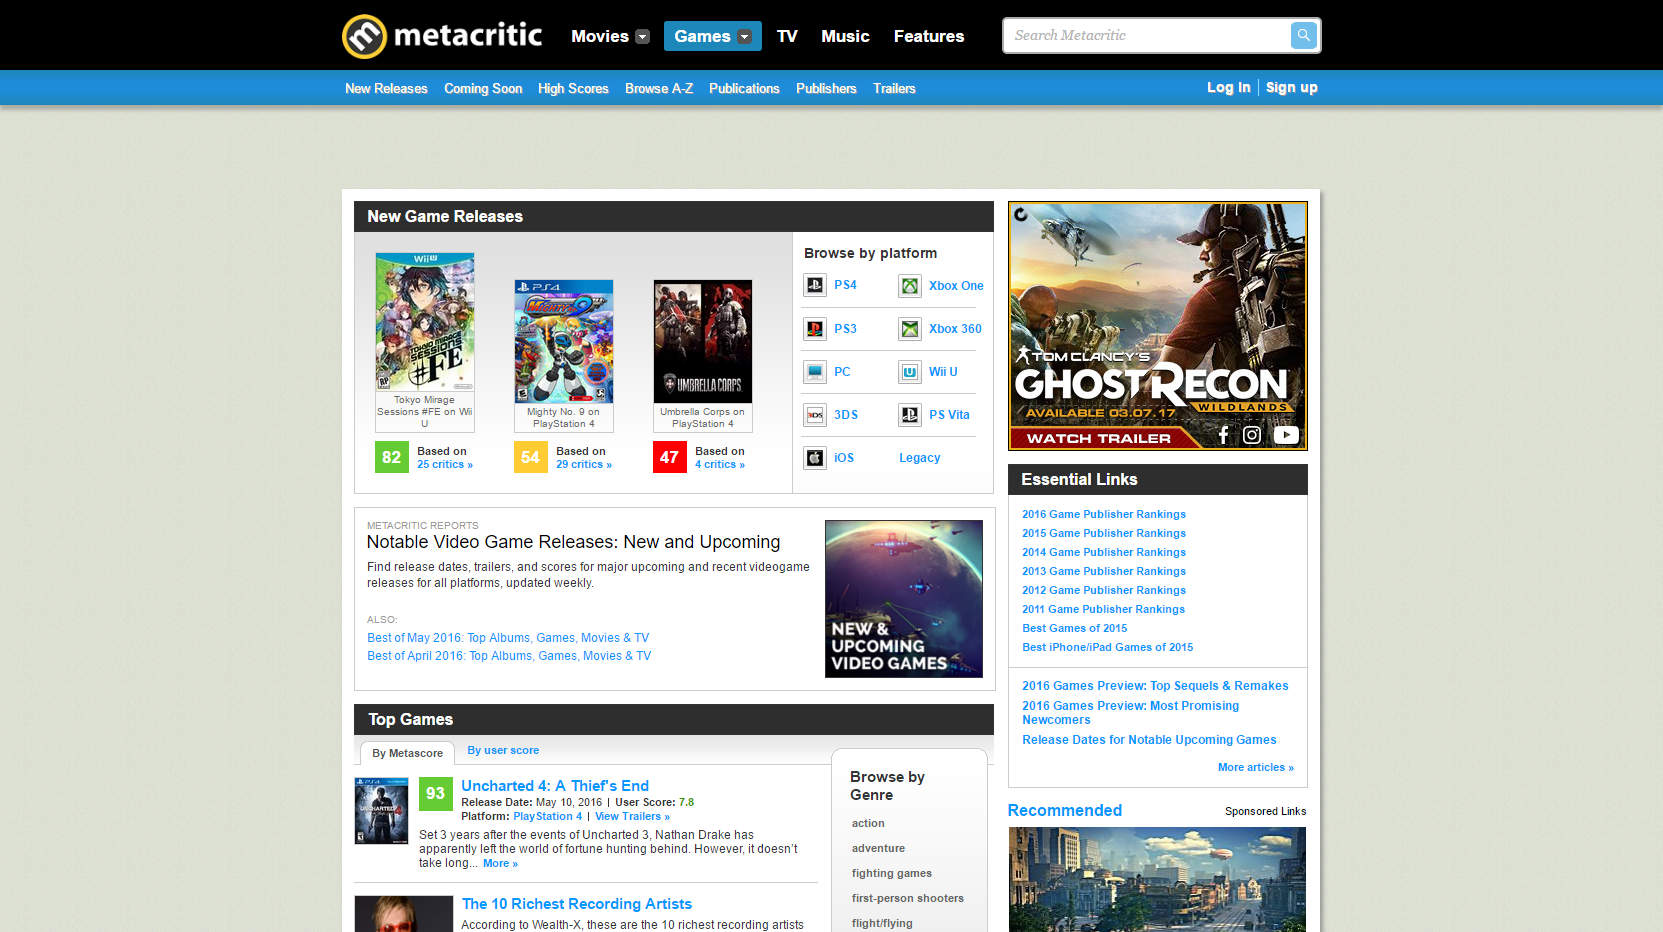
\includegraphics[width=13.5cm]{home2.png}
		\caption{pagina principale games, vedi file \href{home2.png}{home2.png}}
	\end{center}
\end{figure}
\subsection{le sei W}
Si procederà in seguito all'analisi della homepage seguendo le sei W viste a lezione:

\subsubsection{Where}
\textit{Dove sono?}\\
Si nota che è la pagina principale dal fatto che nessuna voce del menu in alo è selezionata.
Infatti se fossimo ad esempio nella sezione movie la barra diverrebbe del tipo:
\begin{figure}[H]
	\begin{center}
		
\includegraphics[width=13.5cm]{menu_non_selezionato.png}
		\caption{vedi file \href{menu_non_selezionato.png}{menu\_non\_selezionato.png}}
	\end{center}
\end{figure}
se vi si passa sopra si apre invece un menu a tendina:
\begin{figure}[H]
	\begin{center}
		
\includegraphics[width=13.5cm]{menu.png}
		\caption{Il menu, vedi file \href{menu.png}{menu.png}}
	\end{center}
\end{figure}
Si noti che nelle pagine specifiche per prodotto compare un secondo menu che porta a pagine con ulteriori funzionalità.
Nota negativa è il fatto che, probabilmente per la struttura particolare del sito, non ci sono breadcrump.
\subsubsection{What}
\textit{Che cosa trovo in questo sito?}\\
Il fatto che si vedano dei numeri di fianco a ogni prodotto fa capire subito che si tratta di un sito che da valutazioni. Da notare che il sito così fa sia capire subito di cosa si occupi sia evita agli utenti fidelizzati un click per scoprire la valutazione del prodotto a cui sono interessati. Inoltre l'uso dei colori per i voti aumenta l'usabilità e la piacevolezza di navigazione. Resta comunque poco chiaro che la valutazione data è il \textit{metascore}.
\subsubsection{Why}
\textit{Perchè dovrei restare su questo sito sito?}\\
Innanzitutto non esistono molti siti che si occupino di organizzare e raggruppare recensioni, soprattutto di recensori professionisti. In aggiunta il \textit{metascore} è una creazione del sito, che per le recessioni professionali è costituito da una media pesata delle recensioni, con un peso per ogni recensione dato dagli amminstratori del sito. Inoltre il team che si occupa di metacritic si occupa anche di trasporre le valutazioni con voti letterali o addirittura senza voto in un voto in base 100, semplificando l'interpretazione delle recensioni. Inoltre è di aiuto per considerare la scelta di acquistare un prodotto consultando le recensioni sia di professionisti sia di utenti comuni, oppure per scegliere un prodotto da acquistare, cercando tra quelli con le recensioni più positive.
\subsubsection{Who}
\textit{chi c'è dietro al sito?}
Il logo è presente correttamente in alto a sinistra, i proprietari del sito sono mostrati nel footer della pagina assieme a dei link per ulteriori informazioni. \'E presente sia una pagina "about us" sia una pagina di FAQ per chiarire altri dubbi riguardo il funzionamento del sito.
\subsubsection{When}
\textit{Cosa c'è di nuovo?}\\
Le novità del sito sono visibili in home. I gestori del sito si occupano di mostrare nella prima pagina i nuovi prodotti con metacritic basandosi sulla loro rilevanza. vi è inoltre all'inizio del corpo della pagina una sezione chiamata "editors' picks" che contiene quelle ritenute in assoluto più rilevanti. Da notare che al di sotto è presente la sezione "new and notable" che mostra i nuovi prodotti degni di nota. Purtroppo si è scelto di utilizzare uno slideshow, che pur essendo gradevole da vedere, risulta poco pratico da utilizzare, tanto più che adempie di più allo scopo la sezione successiva che mostra la lista statica dei nuovi prodotti suddivisi per categoria. Questa parte è purtroppo raggiungibile solamente tramite scroll. Un click su un elemento porta alla corrispondente pagina, mentre un click su "All new .... " avvia una ricerca a campi vuoti sulla categoria selezionata in ordine di data.
\subsubsection{How}
\textit{Come raggiungo ciò che è di mio interesse?}\\
Si è già visto come la barra del menu adempia anche al ruolo di breadcrump surrogato. Consapevoli dell'importanza della ricerca, i gestori del sito hanno implementato una eccellente ricerca, ben visibile in alto a destra, in tempo reale e che ripèrta sia l'icona della lente di ingrandimento sia con il placeholder "Search Metacritic". La ricerca, come si può vedere, è in tempo reale, e inoltre è pure fault tolerant, in quanto permane anche se si sposta il cursore dalla lista dei risultati:
\begin{figure}[H]
	\begin{center}
		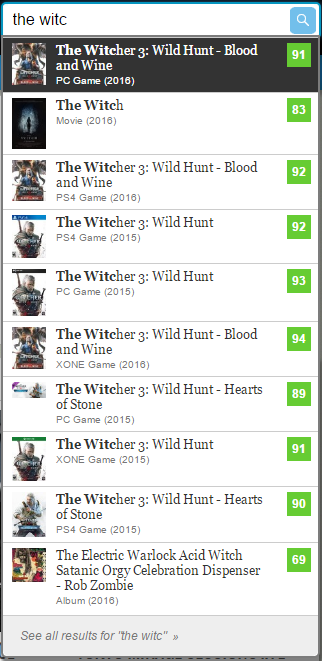
\includegraphics[height=13.5cm]{ricerca.png}
		\caption{Ricerca, vedi file \href{ricerca.png}{ricerca.png}}
	\end{center}
\end{figure}
se si clicca sulla casella "se all results for ...." si viene indirizzati alla seguente pagina:
\begin{figure}[H]
	\begin{center}
		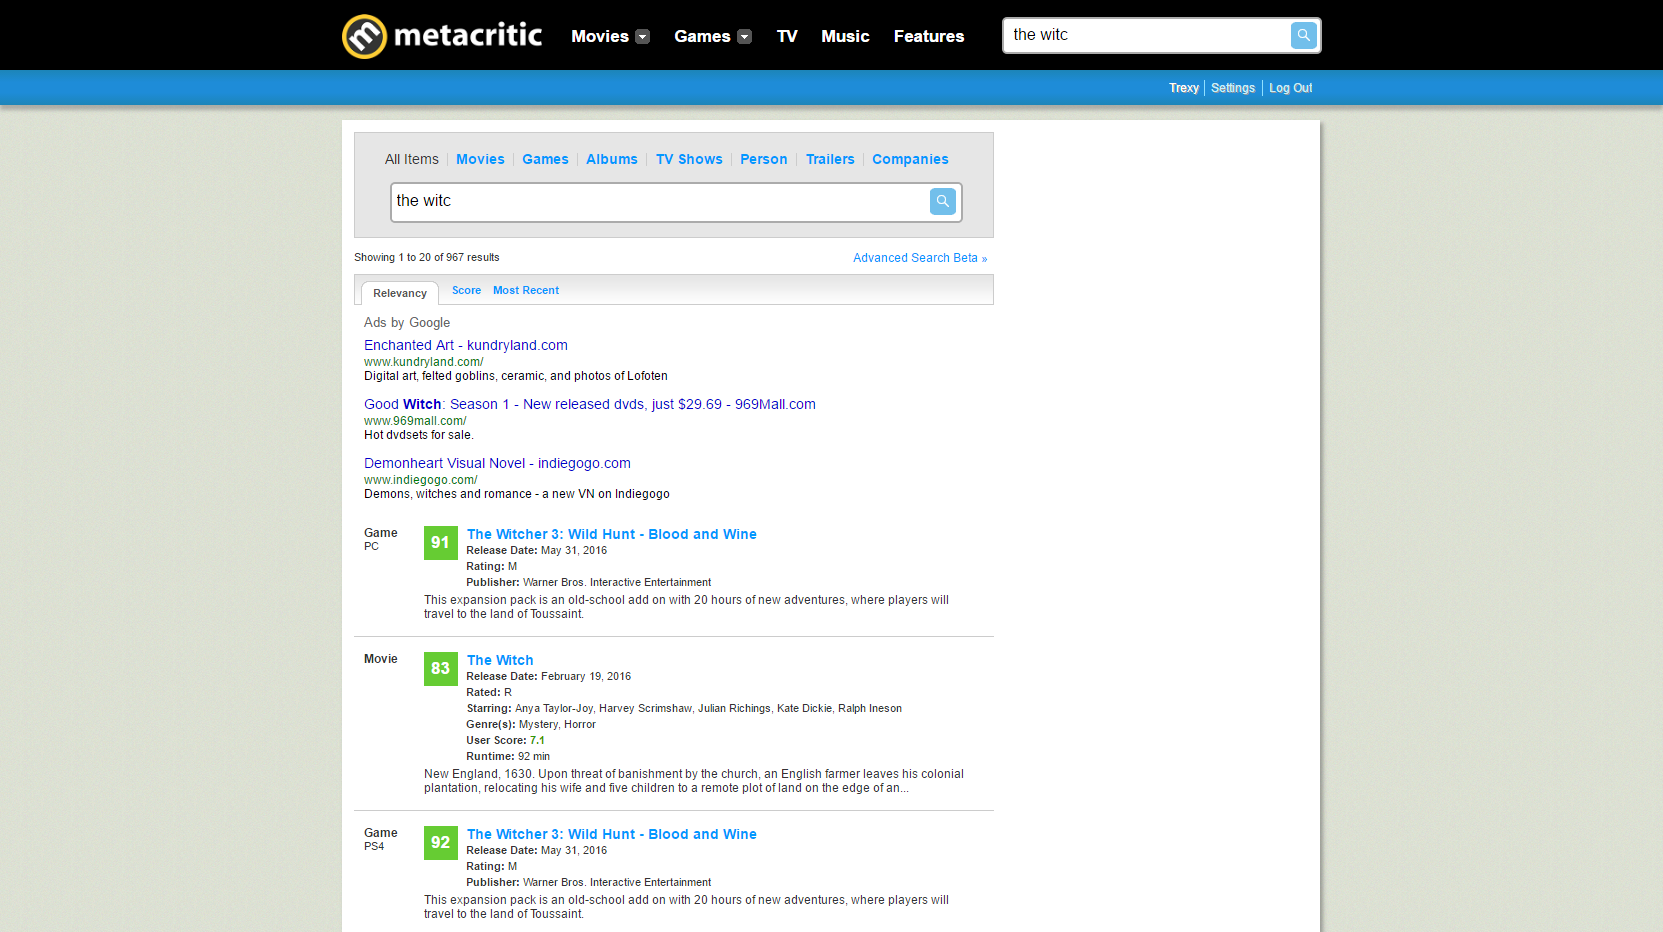
\includegraphics[width=13.5cm]{ricerca2.png}
		\caption{Ricerca, vedi file \href{ricerca2.png}{ricerca2.png}}
	\end{center}
\end{figure}
che offre altre funzionalità quali la ricerca vincolata ad una sola tipologia, e l'ordinamento per data, rilevanza e punteggio, solo in ordine decrescente(basta scorrere al contrario i risultati per la lista inversa).
Da qui è in oltre disponibile un ulteriore raffinamento della ricerca tramite la ricerca avanzata, che offre ancora più vincoli da poter determinare:
\begin{figure}[H]
\begin{center}
	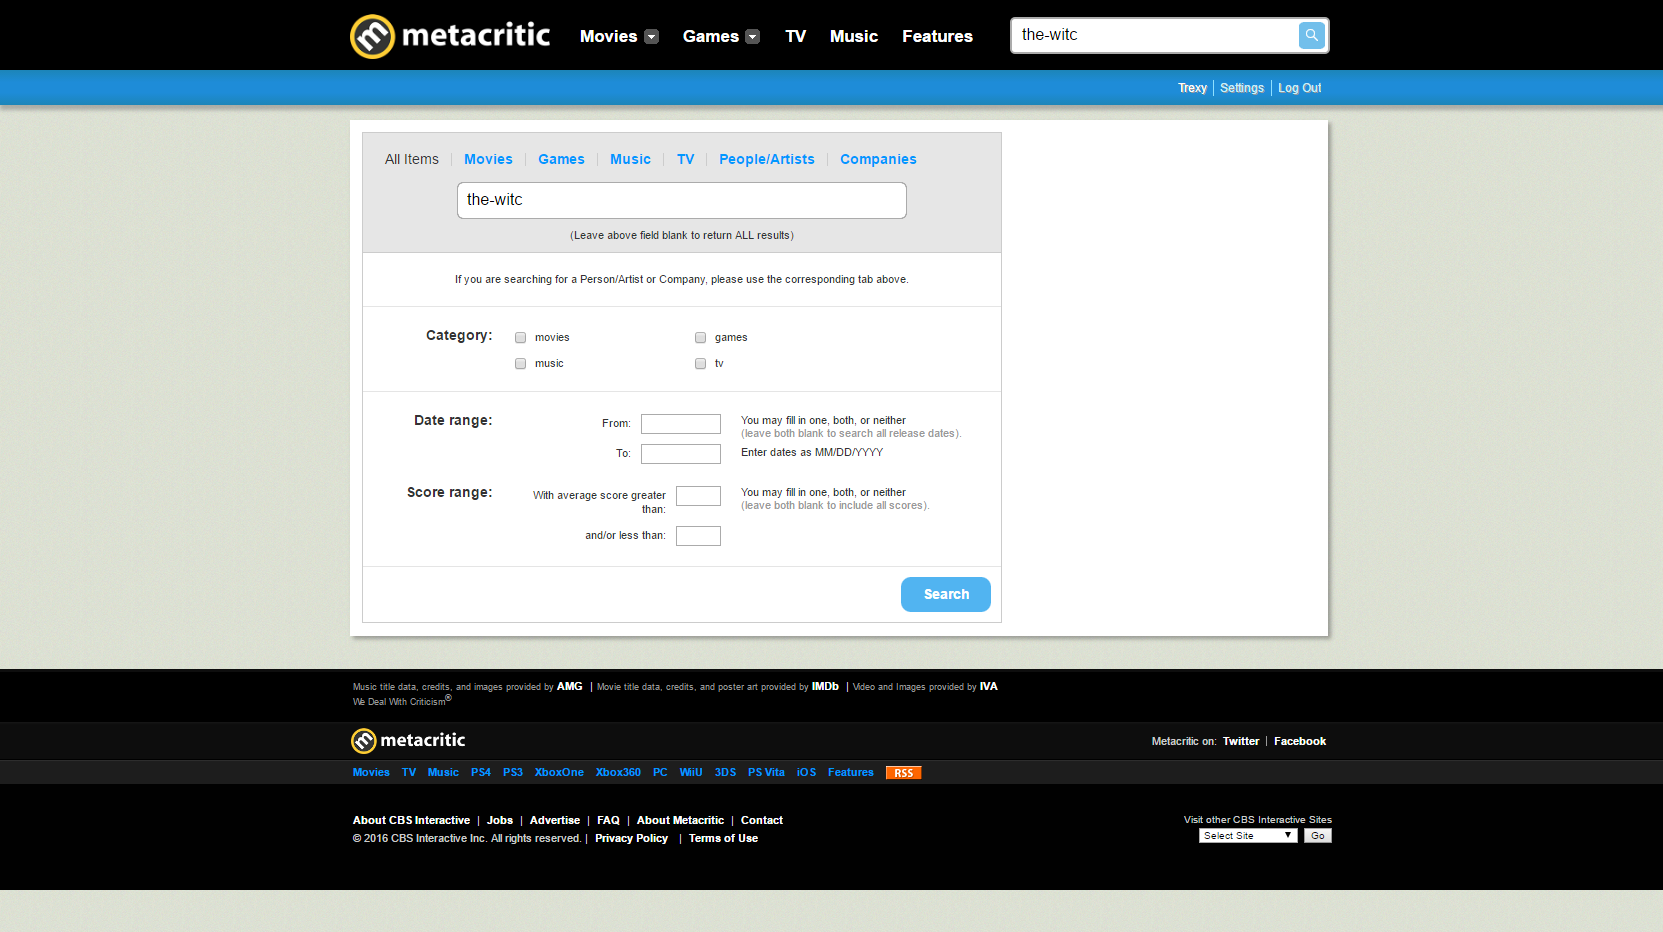
\includegraphics[width=13.5cm]{ricerca3.png}
	\caption{Ricerca avanzata, vedi file \href{ricerca3.png}{ricerca3.png}}
\end{center}
Il comparto ricerca è quindi eccellente, come ci si potrebbe aspettare data la tipologia del sito.
\end{figure}
\newpage
\section{Utenti loggati}
L'esperienza di un utente loggato non cambia molto rispetto a quella di un utente normale, se non per la possibilità di scrivere recensioni e valutare se le recensioni altrui sono state utili per noi o meno. infatti le pagine per un utente sono minimali e principalmente servono a tener traccia delle recensioni e cambiare la propria foto profilo. La scrittura della recensione si va ad integrare con la pagina che visualizza le recensioni degli utenti, ed è semplice ed intuitiva:
\begin{figure}[H]
	\begin{center}
		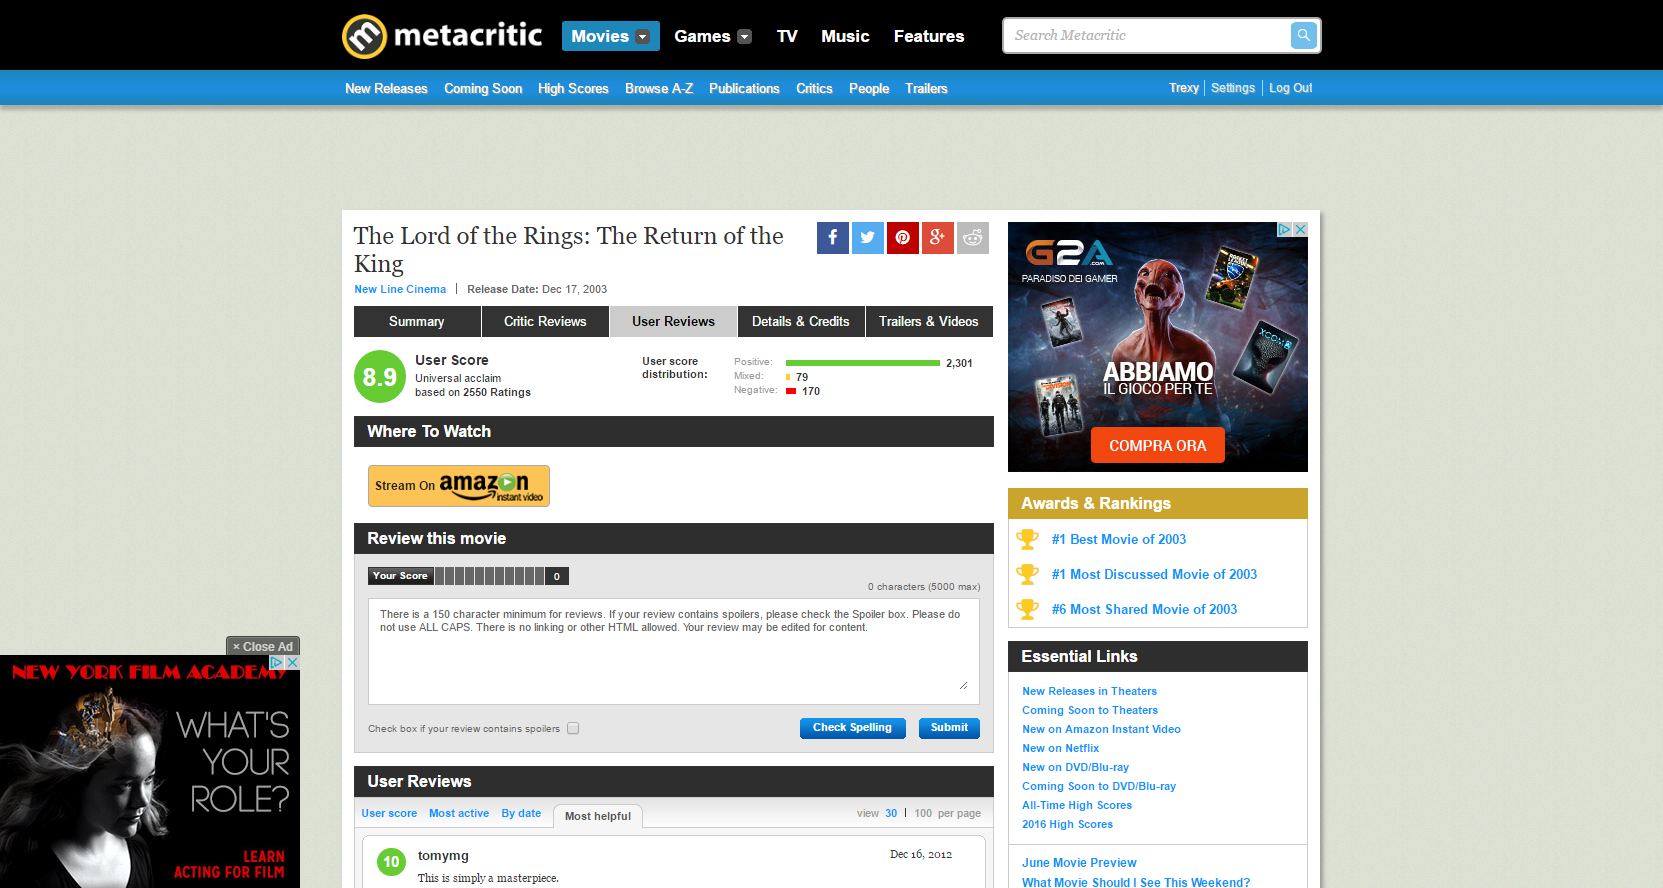
\includegraphics[width=13.5cm]{recensione.png}
		\caption{Scrittura recensione, vedi file \href{recensione.png}{recensione.png}}
	\end{center}
\end{figure}
Inoltre, per ogni utente è possibile vedere la media dei voti che ha dato, il massimo, il minimo e una lista ordinabile per le recensioni. La pagina di un recensore professionista invece è così composta:
\begin{figure}[H]
	\begin{center}
		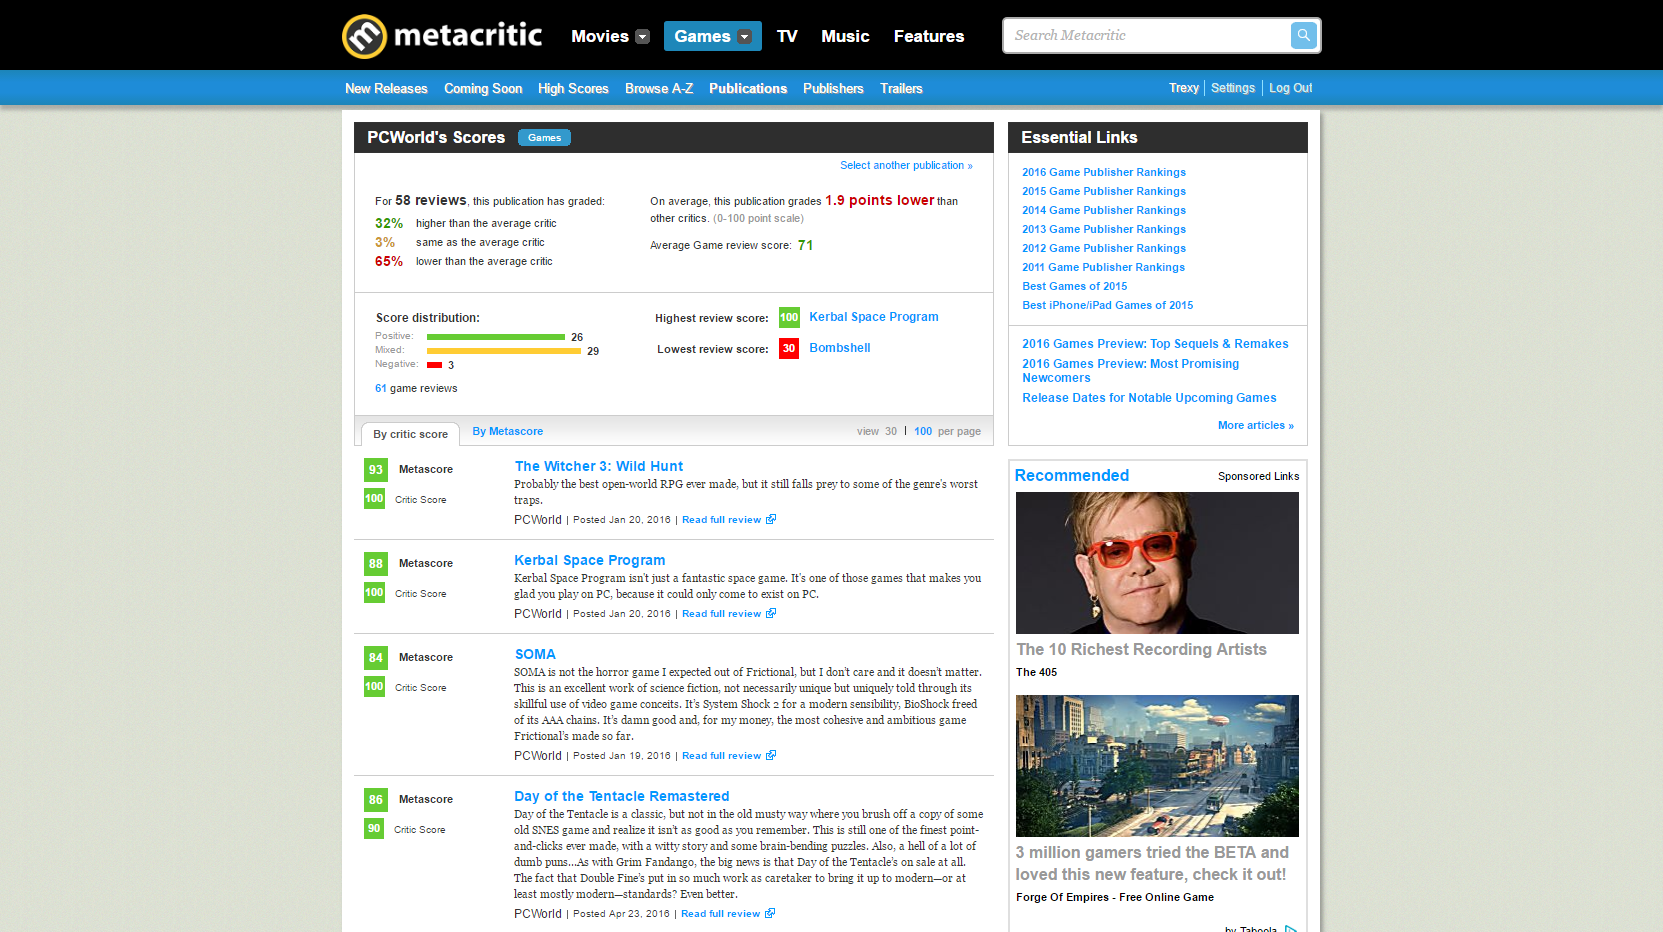
\includegraphics[width=13.5cm]{prof.png}
		\caption{Recensore professionista, vedi file \href{prof.png}{prof.png}}
	\end{center}
\end{figure}
Come si vede è molto snella, utile, e navigabile.
\newpage
\section{Pagina interna}
Si fornisce una pagina di esempio, \url{http://www.metacritic.com/game/pc/the-witcher-3-wild-hunt}, visibile nella sua visione intera in \href{interna1.png}{interna1.png}:
\begin{figure}[H]
	\begin{center}
		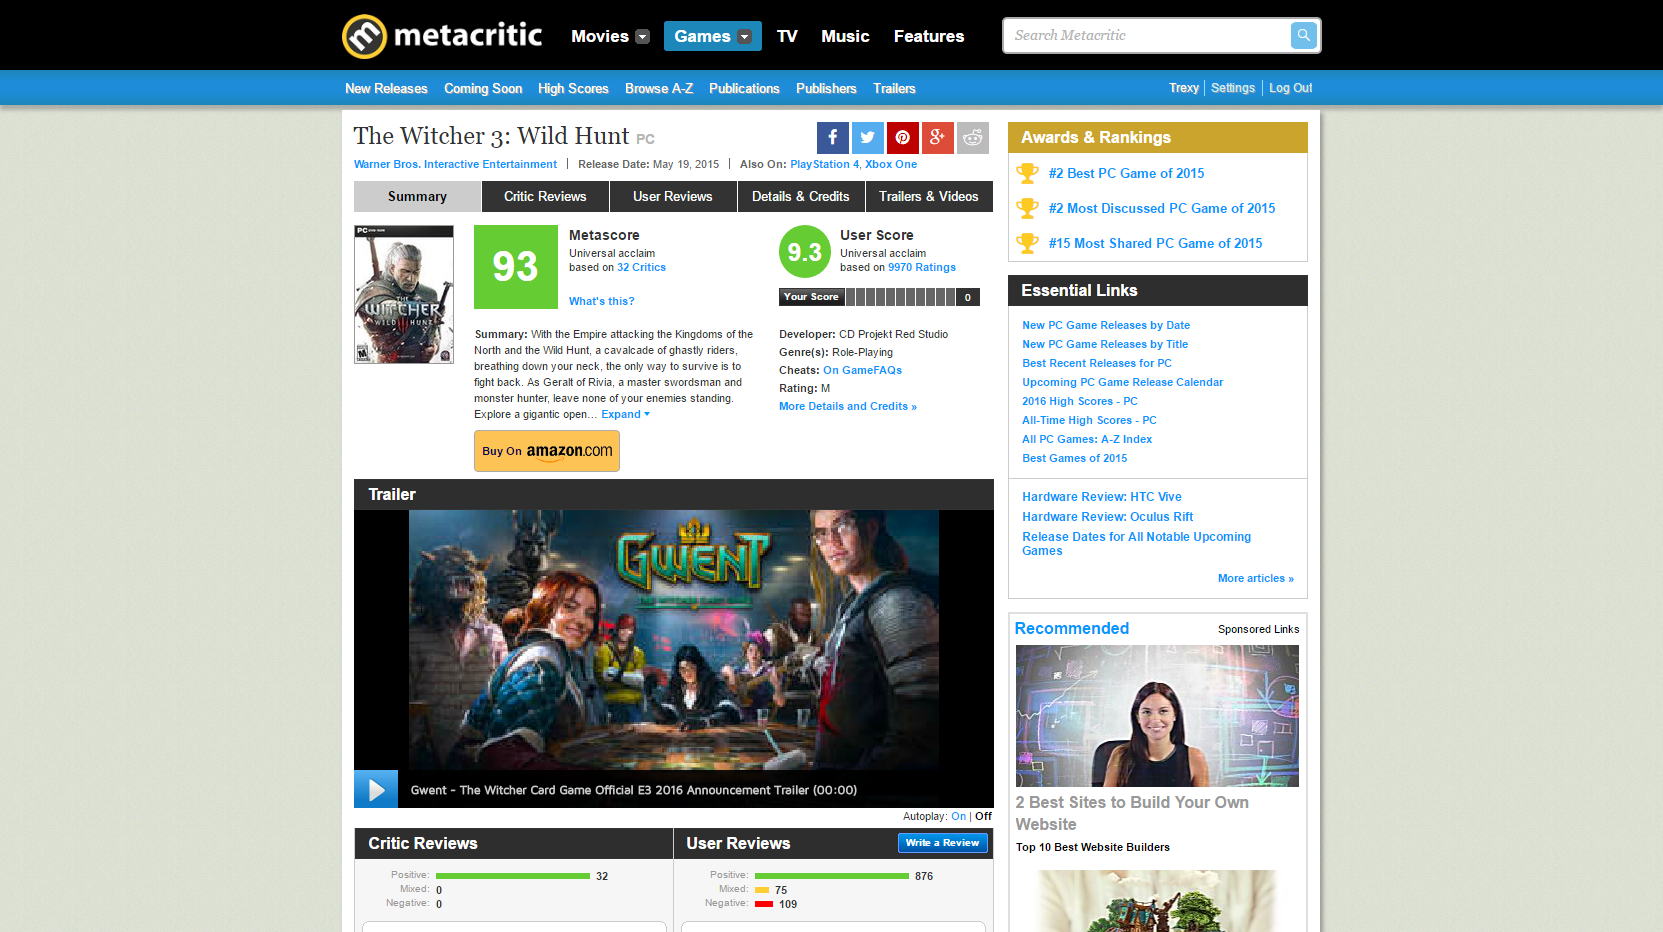
\includegraphics[width=13.5cm]{interna.png}
		\caption{Pagina interna, vedi file \href{interna.png}{interna.png}}
	\end{center}
\end{figure}
Si nota come si cerchi di proporre meno testo possibile, lasciando agli utenti la possibilità di vedere la recensione completa con un ulteriore click, e di mettere in bella vista gli elementi più importanti, quali le valutazioni.
Come si può vedere permangono immutati tutti gli assi a parte il where, che è qui ridotto ad una lista sulla colonna di destra degli elementi più recenti
\newpage
\section{Pubblicità}
Le pubblicità, sia nelle pagine interne che in quelle principali, sono situate in tutte le posizioni possibili: in alto prima del contenuto, alla fine, a sinistra, a destra e anche mimetizzata nel contenuto. Le pubblicità a volte risultano tagliate o il box che le contiene è sovradimensionato oppure addirittura non compaiono sprecando spazio e facendo calare drasticamente la piacevolezza di navigazione. Un esempio è il seguente:
\begin{figure}[H]
	\begin{center}
		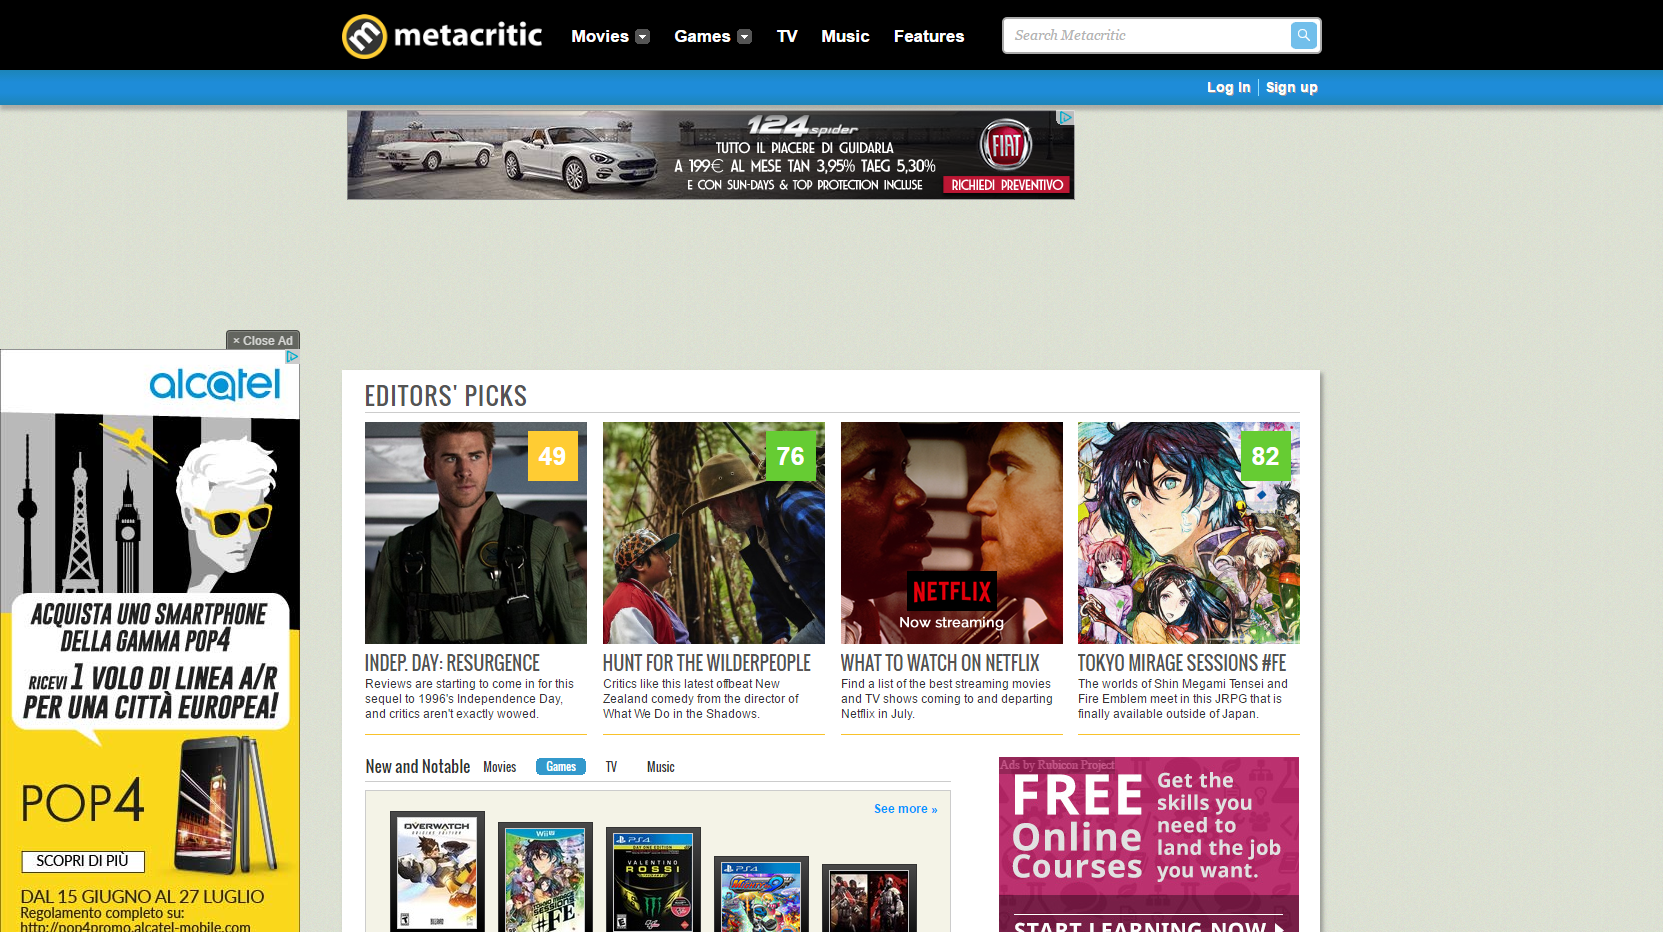
\includegraphics[width=13.5cm]{ads.png}
		\caption{vedi file \href{ads.png}{ads.png}}
	\end{center}
\end{figure}
Nelle pagine interne come si poteva vedere nelle immagini mostrate prima, è presente un pulsante in cui è possibile guardare in streaming o comprare il prodotto sul noto sito di e-commerce \textit{Amazon}. Questo pulsante, se da una parte è utile per l'utente e comporta guadagno per il sito data la collaborazione biunivoca tra le due parti (Amazon riporta il metascore con tanto di link a metacritic sui videogiochi che vende), dall'altro comporta un gambling click, in quanto si è inspiegabilmente scelto di non riportare il prezzo, come invece è fatto da molti altri siti che integrano la funzionalità del pulsante "buy on Amazon"
Le pubblicità del sito fanno uso di \textit{Google AdSense} per personalizzare le pubblicità che si presentano all'utente, aumentando di molto la piacevolezza di queste.
La piacevolezza della navigazione aumenta utilizzando un \textit{adblocker}, che comunque non blocca tutte le pubblicità, segno che i gestori del sito hanno lavorato per contrastarlo.
\newpage
\section{errore 404}
di seguito è riportata l'immagine di cosa comporta generare un errore 404:\\
\begin{figure}[H]
	\begin{center}
		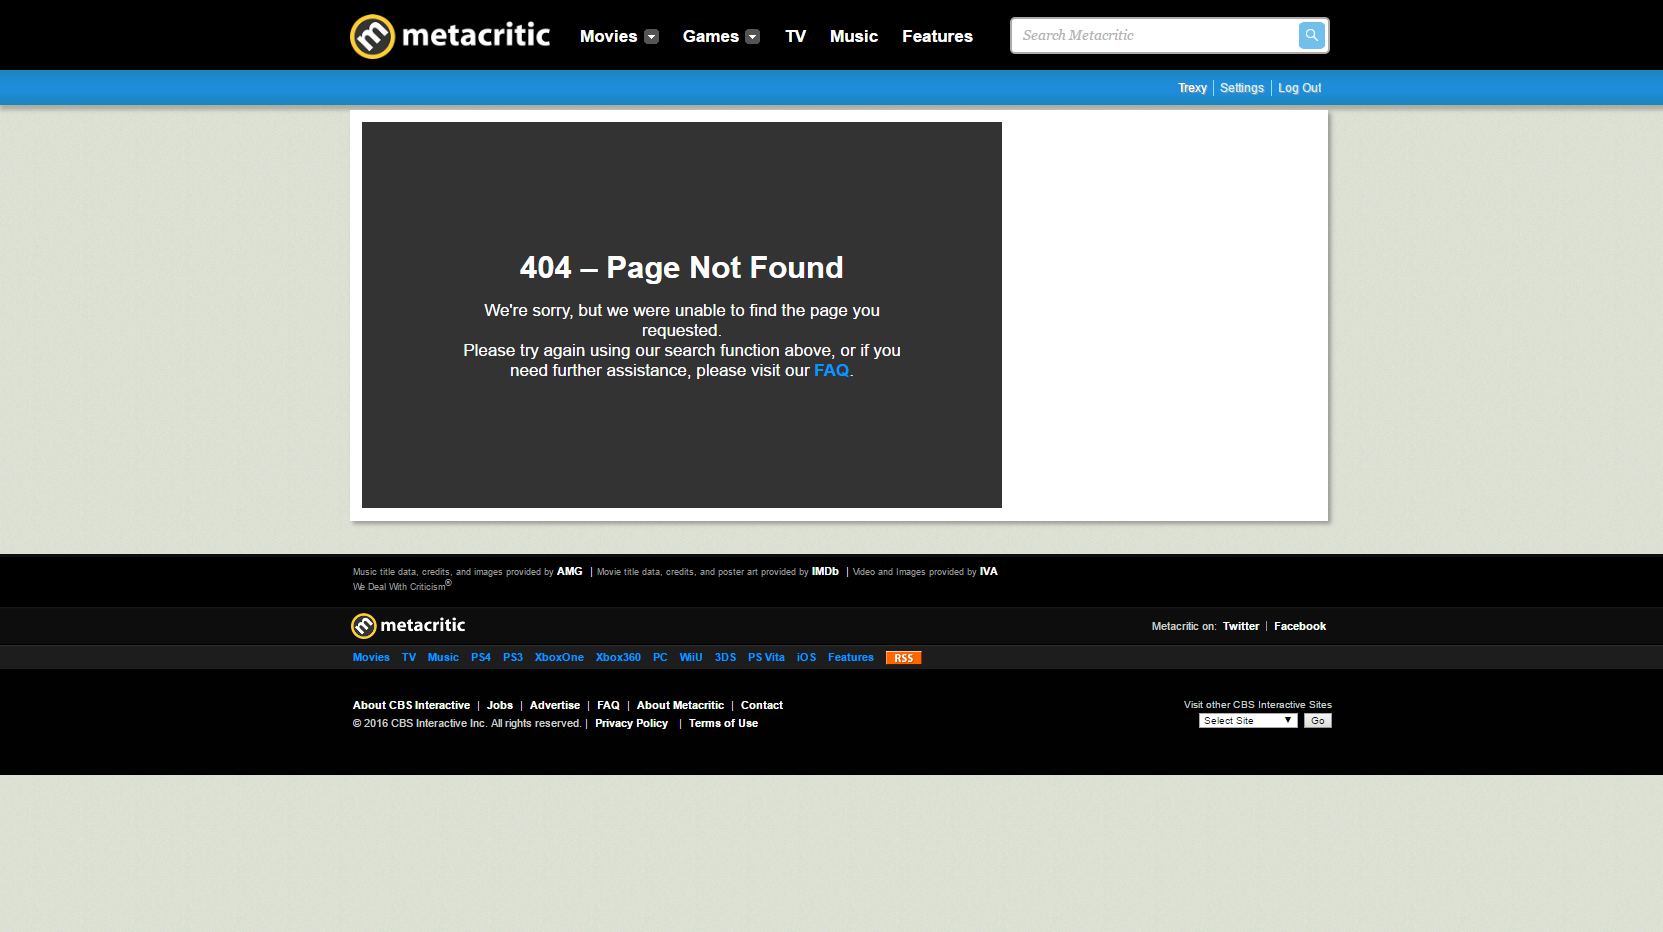
\includegraphics[width=13.5cm]{404.png}
		\caption{errore 404, vedi file \href{404.png}{404.png}}
	\end{center}
	come si vede, il messaggio è serio e significativo, e incita a leggere le FAQ o ad utili
\end{figure}
\newpage
\section{layout mobile}
per completezza, si riporta anche uno screen del layout mobile. Il menu compare alla pressione del tasto in alto a sinistra e la ricerca con la pressione dell'icona della lente di ingrandimento.
La barra di ricerca è larga quanto lo schermo e compare sotto al menu. Non ci sono constatazioni particolari da aggiungere rispetto a quanto detto. Risulta più piacevole da navigare rispetto a quella desktop, in quanto ad esempio vengono tolti gli inutili orpelli quali lo slideshow.
\begin{figure}[H]
	\begin{center}
		
\includegraphics[width=7cm]{mobile.png}
		\caption{Layout mobile, vedi file \href{mobile.png}{mobile.png}}
	\end{center}
\end{figure}
\section{Giudizio finale}
In conclusione, tenendo conto che la funzionalità di ricerca è eccellente e del fatto che il sito è pensato soprattutto per una categoria di utenti che sa quello che vuole e non si sofferma alla home e va dritta al dunque, si ritiene di non dover penalizzare oltre il dovuto le mancanze della home e delle carenze di navigazione. Rimangono molto pesanti però le pubblicità, che a tratti sovrastano il testo e impattano l'usabilità. Ritengo di poter assegnare al sito un voto pari a
	\begin{center}
		\huge 8/10
	\end{center}
	\newpage
	\section{lista delle figure}
	\'E in seguito riportata la lista delle figure che sono state utilizzate in questo rapporto.
	\begin{itemize}
	\item \href{home.png}{home.png} e \href{home1.png}{home1.png}: sono la home page, \url{http://www.metacritic.com/}
	\item \href{home.png}{home2.png} e \href{home.png}{home21.png}: sono la pagina principale della sottosezione games, \url{http://www.metacritic.com/game}
	\item \href{ricerca2.png}{ricerca2.png}: ricerca, vedi pagina \url{http://www.metacritic.com/search/all/the\%20witc/results}
	\item \href{ricerca3.png}{ricerca3.png}: ricerca avanzata, vedi pagina  \url{http://www.metacritic.com/advanced-search/all/the+witc}
	\item \href{recensione.png}{recensione.png}: vedi pagina http://www.metacritic.com/movie/the-lord-of-the-rings-the-return-of-the-king/user-reviews da loggato
	\item \href{prof.png}{prof.png}: vedi pagina \url{http://www.metacritic.com/publication/pcworld?filter=games}
	\item \href{interna.png}{interna.png}: pagina interna, vedi \url{http://www.metacritic.com/game/pc/the-witcher-3-wild-hunt}
	\item \href{ads.png}{ads.png}: è la home page, ma il risultato non è replicabile con un link.
	\item \href{404.png}{404.png}: errore 404, basta far lanciare un errore 404. Non si forniscono link in quanto l'indirizzo utilizzato potrebbe corrispondere a una risorsa in futuro.
	\item \href{mobile.png}{mobile.png}: è la home page vista da mobile.
	\end{itemize}
		Le altre immagini utilizzate sono ritagli delle pagine già citate.
\end{document}